\documentclass[times, utf8, zavrsni]{fer}
\usepackage{booktabs}
\usepackage{algorithm,algpseudocode}
\usepackage{lipsum}

\begin{document}

% TODO: Navedite broj rada.
\thesisnumber{688}

% TODO: Navedite naslov rada.
\title{Evolving cache replacement policies using grammatical evolution}

% TODO: Navedite vaše ime i prezime.
\author{Mihael Miličević}

\maketitle

% Ispis stranice s napomenom o umetanju izvornika rada. Uklonite naredbu \izvornik ako želite izbaciti tu stranicu.
\izvornik

% Dodavanje zahvale ili prazne stranice. Ako ne želite dodati zahvalu, naredbu ostavite radi prazne stranice.
\zahvala{}

\tableofcontents

\chapter{Introduction}

Genetic programming is a branch of evolutionary computing whose primary concern is evolving computer programs, usually starting from random populations of programs. The evolution of these programs is inspired by the Darwinian theory of natural evolution, which lies on five basic principles \citep{cupic2019evolucijskoracunarstvo}:

\begin{enumerate}
	\item There are always more offspring than necessary.
	\item The size of the population is approximately constant.
	\item The quantities of the food resources are limited.
	\item Species which sexually reproduce bear no identical offspring, instead there are always variations.
	\item Most of these variations are hereditary.
\end{enumerate}

One of the main tools in compiler design are context-free grammars. They provide an elegant, formal way of describing the structural rules of computer programs, and each valid computer program written in some arbitrary language satisfies the rules of that language's grammar. Grammar-based approaches in the field of genetic programming have enjoyed much popularity \citep{neill2003grammaticalevolution}, and the most popular and used technique is the grammatical evolution.

The topic of this thesis is using grammatical evolution in solving a popular benchmarking problem in the field of genetic programming, which is evolving cache replacement policies. The rest of this thesis is organised as follows: chapter 2 covers the theoretical background involved in solving this problem, chapter 3 explains the problem of cache replacement policies and how it can be solved using grammatical evolution, chapter 4 covers the experiment design and the results analysis, and chapter 5 covers a conclusion of the thesis. Finally, in the appendix A, the software system constructed for the experiments covered in chapter 4 is described in detail.

\chapter{Theoretical background}

\section{Context-free grammars}
\subsection{Formal definition}
A formal grammar is a 4-tuple $G = (V, T, P, S)$ \citep{sipser2013introduction} where
\begin{list}{$\bullet$}{}  	
	\item $V$ is a finite set of nonterminal symbols.
	\item $T$ is a finite set of terminal symbols, disjoint from $V$.
	\item $P$ is a finite set of production rules that represent the recursive definition of a language. Each production has three components \citep{hopcroft2007automatatheory}:
		\begin{list}{$\circ$}{}
			\item head, which consists of one or more terminal and nonterminal symbols.
			\item production symbol $\rightarrow$.
			\item body, which consists of zero or more terminal and nonterminal symbols. If the body is empty (if it consists of zero symbols), we denote that by writing $\epsilon$.
		\end{list}
	\item $S$ is the start nonterminal symbol.
\end{list}

We can think of the terminal $T$ and nonterminal $V$ symbols as the building blocks of the grammar. Productions $P$ define the rules by which these building blocks substitute each other in the process of building a string. This string belongs to the language which is defined by the grammar. The start symbol $S$ represents the starting building block. The process of building a string starts by applying a production over the start symbol, and this process of applying productions over intermediate strings continues until no more productions can be applied. At that point, the result string is built, and it consists only of the elements of the $T$ set, which belong to the alphabet of the language.

\subsection{Formal grammar types}
The most general grammars, defined only by the aforementioned rules and with no other restrictions, are called unrestricted grammars. For example, we can define one unrestricted grammar as $G = (\{A, B, C\}, \{a, b, c, d\}, P, A)$ where $P$ contains productions such as:
\begin{list}{$\bullet$}{}  	
	\item $AB \rightarrow c$
	\item $aBdC \rightarrow \epsilon$
	\item $a \rightarrow ABdCAB$
	\item $abba \rightarrow ABBA$
\end{list}

Context-free grammars are a subset of unrestricted grammars which impose one additional restriction, that the head of a production is exactly one symbol from the nonterminal symbols $V$. With this restriction, none of the previously written productions can be valid in a context-free grammar, but we can write productions such as:
\begin{list}{$\bullet$}{}  	
	\item $A \rightarrow \epsilon$
	\item $B \rightarrow a$
	\item $A \rightarrow abCdB$
	\item $C \rightarrow abba$
\end{list}

Context-free grammars get their name from their property that every nonterminal symbol $A$ from $V$ can be substituted with a string of terminals and nonterminals $S$ if there exists a production rule in $P$ such that $A \rightarrow S$, no matter its surrounding context in the intermediate string.

Context-free grammars have played a central role in the development of the compiler technology \citep{hopcroft2007automatatheory}. They are used to define the syntax rules of a language, as they are expressive enough to allow recursions, nesting and other concepts we expect from programming languages, yet they are simple enough to be parsed effectively.

\section{Genetic algorithm}
Genetic algorithm is a metahueristic inspired by the Darwinian theory of evolution. The main idea is that, given a population in an environment with limited resources, competition for those resources causes natural selection \citep{eiben2015evolutionarycomputing}.  This principle is sometimes called 'survival of the fittest'. 

One of the first design choices in solving an optimisation problem using a genetic algorithm is individual representation. We can distinguish two different terms - genotype and phenotype. Genotype corresponds to the encoding of an individual. Variation operators (recombination and mutation) are applied on the genotype of an individual. In the process of evaluating an individual, it's genotype is decoded onto it's phenotype. Phenotype corresponds to the actual solution, and we determine how good of a solution one individual is by evaluating it's phenotype using a fitness function.

The basic idea flow of a genetic algorithm is described as \citep{eiben2015evolutionarycomputing}:

\begin{algorithm}[]
\caption{Genetic algorithm}
\begin{algorithmic}[1]
\State $\text{initialise } \textit{population} \text{;}$
\State $\text{evaluate } \text{each solution};$
\State $\text{repeat while (} \textit{terminal condition} \text{ not satisfied)}$
\State $\indent \text{select } \textit{parents} \text{;}$
\State $\indent \text{recombine pairs of } \textit{parents} \text{;}$
\State $\indent \text{mutate acquired } \textit{children} \text{;}$
\State $\indent \text{evaluate } \textit{children} \text{;}$
\State $\indent \text{select individuals for next generation;}$
\end{algorithmic}
\end{algorithm}

In line 1, we initialise the population. We can either initialise it with random solutions, or, if we know some good solutions which can be a good starting point for the evolutionary search process, we can seed it with those.

In line 2, we evaluate each solution using a fitness function. Fitness function is applied over the individual's phenotype, and it returns a measure of how good a solution is. In that case, the goal of the genetic algorithm is to find the solutions which maximize this measure. When solving some problems, it is much easier to determine how bad of a solution one individual is, rather than how good of a solution it is. In that case, fitness function returns a measure of how bad a solution is, and the goal of the genetic algorithm is to minimize this measure.

In line 3, we start the evolutionary loop. Each new iteration of this loop corresponds to a different generation of the population. This loop is stopped when some stopping criteria is satisfied. The simplest stopping criteria is reaching the predetermined number of iterations. If we know how good of a solution we need, we can also stop this loop once we find one such solution.  

In line 4, we select the parents which we will later recombine to get their offspring, which will be new candidate solutions. When choosing which individuals will be parents, we want to keep their fitness in mind. We want to choose the better individuals more often, in order to guide the evolutionary search towards better solutions. If we don't discriminate individuals over their fitness when selecting parents for future solutions, our evolutionary search can degrade into random search. On the other hand, we want to be able to choose the bad solutions to be parents as well, albeit with a low chance. If we chose only the good solutions to be parents, our search could become too greedy, and get stuck in a local optimum.

In line 5, we recombine the genotype of selected parents to get the genotype of their offspring. Recombination process can yield one or more offspring. The idea behind recombination is - if we chose a good genotype-phenotype mapping, we can expect that an individual's fitness will be coded into it's genotype. Combining good solutions should yield even better solutions, if we choose the good parts of the first parent and good parts of the second parent, and then combine these good parts into a new solution. Of course, since the recombination process is random, we can also sometimes choose the bad part of the first parent and the bad part of the second parent to get an individual that is worse than it's parents, but that isn't a significant problem, since we can also get good solutions which can guide the evolutionary search.

In line 6, we apply the mutation operator on newly constructed individuals, which are the result of the recombination process. The main idea behind mutation is that it should increase diversity of the population. Mutation operator should not be guided by some rule, instead, it should be random and unbiased \citep{eiben2015evolutionarycomputing}. If we don't include the mutation operator, or if we set the mutation rate to be too low, our search can get stuck in a local optimum. On the other hand, we don't want the mutation rate to be too large either. Since the new solutions are constructed from good solutions (with a high chance), and we expect that good solutions have their fitness coded into their genotypes, if the mutation operator is too disruptive, it can nullify the good results of the recombination, and degrade our evolutionary search into random search. 

In line 7, we evalute newly construced individuals. These individuals are being evaluated with the same fitness function used in line 2.

In line 8, we choose which individuals carry on to the next generation. Unlike the parent selection, which is stochastic, this process is usually deterministic. Two common strategies are choosing the best individuals from both parents and offspring, and the age-biased approach, which chooses only from the offspring \citep{eiben2015evolutionarycomputing}. If we choose the latter approach, a problem we might encounter is loosing good solutions, if these good solutions have no children better than themselves. To counter this problem, we can choose to carry over a few of the best solutions into the next generation without changing them, and this approach is called elitism.

\section{Grammatical evolution}
\subsection{Definition}
Grammatical evolution is a evolutionary computation technique used to evolve computer programs which have a high fitness in regards to a fitness function, or in other words, which do some certain task well. The phenotypes of the individuals are executable computer programs. The genotypes of the individuals are arrays of 8-bit numbers, called codons. Authors of the algorithm have propposed using 8-bit codons in \citep{neill2003grammaticalevolution}. They've also ran some experiments with 12-bit codons and 16-bit codons, and the results have shown that increasing the codon size can result in slower evolutionary search. The genotype-phenotype mapping is done using a context-free grammar which generates the language of the desired solutions.

The process of the genotype-phenotype mapping works as follows: we start at the first codon in individual's genotpye, and we traverse the parsing tree using depth-first search, until we find a nonterminal symbol. Once we find a nonterminal symbol, we check all productions of our specified grammar in which this nonterminal symbol is the left side (head). We calculate which production to apply on this nonterminal symbol using the formula
$$Production\:=\:(Codon\:integer\:value)$$
$$MOD$$ 
$$(Number\:of\:productions\:for\:the\:current\:nonterminal\:symbol)$$ 

Once we apply the chosen production, we move on to the next codon. If we have reached the end of codon array, we move to the first codon, and this process is called wrapping. In practice, the maximum number of wrappings is specified, in order to avoid infinite recursions, and if the process exceeds this maximum number of wrappings, the mapping fails and the individual's fitness is set to the lowest possible value.

This process of traversing the parsing tree and applying grammar productions continues until there are no more nonterminal symbols in the parsing tree, and at that point the mapping is complete \citep{neill2003grammaticalevolution}.

\subsection{Properties}
Grammatical evolution has some interesting unique properties, namely the wrapping operator and code degeneracy \citep{neill2003grammaticalevolution}. 

During the genotype-phenotype mapping process, an individual could run out of codons. In that situation, the wrapping operator is applied, which means that the mapping continues from the first codon. This technique draws inspiration from a phenomen exhibited by bacteria, viruses and mitochondria which allows them to reuse the same genetic material for the expression of different genes \citep{neill2003grammaticalevolution}.

Code degeneracy refers to the fact than the mapping process used in grammatical evolution is many-to-one. Many different codon configurations in the genotype can map onto the same phenotype program. For example, during the mapping process, if the current nonterminal symbol has two different productions as specified by the grammar, then the first production would be chosen if the current codon value is even, and the second production would be chosen if the current codon value is odd. This is because $0\:MOD\:2\:=2\:MOD\:2\:=4\:MOD\:2\:=6\:MOD\:2\:=\:...\:=254\:MOD\:2\:=0$, and $1\:MOD\:2\:=3\:MOD\:2\:=5\:MOD\:2\:=7\:MOD\:2\:=\:...\:=255\:MOD\:2\:=1$. The values are shown up to 254 and 255 because these are the largest even and odd numbers, respectively, that fit into the 8 bits of one codon. This property of the genotype-phenotype mapping which enables it to have many different genotypes which all map to the same phenotpye cultivates the genetic diversity of the population \citep{neill2003grammaticalevolution}.

Grammatical evolution has some drawbacks, namely low locality and high redundancy. Low locality refers to the property of the genotype-phenotype mapping that small changes in genotype can cause drastic changes in phenotype, or even completely different phenotypes. High redundancy refers to the fact that the genotype-phenotype mapping is many-to-one, which means that many different genotypes can map to a single phenotype. Because of these two properties, the evolutionary search process in grammatical evolution can sometimes behave like random search \citep{megane2022coevolutionary}. To solve these problems, some extensions of the standard grammatical evolution have been proposed, like the structured grammatical evolution \citep{lourenco2018structured}.

\subsection{Demonstration of the genotype-phenotype mapping process}
To demonstrate the process of the genotype-phenotype mapping in the grammatical evolution, we will define a context-free grammar and one individual's genotype, and then show a step by step mapping from the genotype to the phenotype. Instead of defining a grammar using the $(V, T, P, S)$ 4-tuple, we will define it using the BNF notation. Terminal symbols are written as lowercase symbols, nonterminal symbols are written as uppercase symbols surrounded by the symbols '<' and '>', and the first nonterminal symbol is the start symbol. Production heads are written on the left side of the '::=' string, and on the right side of this string are bodies of productions which share their left side, separated by the symbol '|'. We will define our grammar as:

\noindent
$ {<}S{>}\:::=\:a\:{<}A{>}\:b\:{<}S{>}\:|\:{<}C{>}\:d\:{<}A{>}\:$\\
$ {<}A{>}\:::=\:c\:{<}B{>}\:{<}A{>}\:c\:|\:a\:b\:{<}C{>}\:|\:d $\\
$ {<}B{>}\:::=\:{<}S{>}\:a\:{<}S{>}\:|\:{<}C{>}\:d\:{<}A{>}\:|\:b\:d $\\
$ {<}C{>}\:::=\:c\:{<}C{>}\:|\:{<}C{>}\:d\:{<}C{>}\:|\:a $\\

We will also define one individual with the genotype: 
$$ [\:176,\:49,\:168,\:253,\:8,\:65,\:127,\:26,\:130,\:100\:] $$

All the intermediate strings will be displayed like linear strings, which can be constructed by traversing the parsing tree in depth.

Each step of the mapping process will be followed by a figure showing the current state of the process visually. On the top of all figures is the unit's genotype shown as a array. All the fields in this array are colored ih blue, except for the one which the index used in mapping at this turn points to, as this field is colored in yellow. Beneath the genotype array will be the parsing tree built up to that point. The nonterminal symbol which will be expanded at this turn is colored in red. The nonterminal symbols which have already been expanded are colored in green, and the nonterminal symbols which haven't yet been expanded and won't be at this turn, but sometime later in the future are colored in orange. Finally, the leaves of the tree, which are the terminal symbols, are colored in brown. These figures were built using the tool \citep{diagrams}.

The mapping process starts with the string ${<}S{>}$, and the index $i = 0$ in the genotype array. Since $i = 0$, the codon value we will use at this step is $176$. The first nonterminal symbol in the string is ${<}S{>}$, and it has $2$ productions defined in the grammar. So we calculate $176\:\:MOD\:\:2\:=\:0$, and apply the production at index $0$, which is ${<}S{>}\:::=\:a\:{<}A{>}\:b\:{<}S{>}$.

\begin{figure}[H]
	\centering
	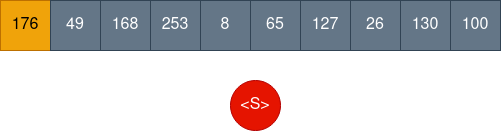
\includegraphics[scale=0.6]{parsing_tree_01.png}
	\caption{Genotype-phenotype mapping, step 1}
\end{figure}

Our current string is $a\:{<}A{>}\:b\:{<}S{>}$, the index value is $i = 1$, and the codon value is $49$. The leftmost nonterminal symbol is ${<}A{>}$, which has $3$ productions defined. So we calculate $49\:\:MOD\:\:3\:=\:1$, and apply the production at index $1$, which is ${<}A{>}\:::=\:a\:b\:{<}C{>}$

\begin{figure}[H]
	\centering
	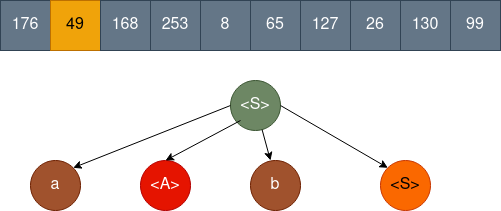
\includegraphics[scale=0.6]{parsing_tree_02.png}
	\caption{Genotype-phenotype mapping, step 2}
\end{figure}

Our current string is $a\:a\:b\:{<}C{>}\:b\:{<}S{>}$, the index value is $i = 2$, and the codon value is $168$. The leftmost nonterminal symbol is ${<}C{>}$, which has $3$ productions defined. So we calculate $168\:\:MOD\:\:3\:=\:0$, and apply the production at index $0$, which is ${<}C{>}\:::=\:c\:{<}C{>}$.

\begin{figure}[H]
	\centering
	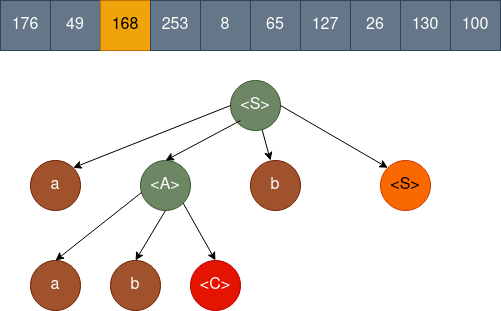
\includegraphics[scale=0.6]{parsing_tree_03.png}
	\caption{Genotype-phenotype mapping, step 3}
\end{figure}

Our current string is $a\:a\:b\:c\:{<}C{>}\:b\:{<}S{>}$, the index value is $i = 3$, and the codon value is $253$. The leftmost nonterminal symbol is ${<}C{>}$, which has $3$ productions defined. So we calculate $253\:\:MOD\:\:3\:=\:1$, and apply the production at index $1$, which is ${<}C{>}\:::=\:{<}C{>}\:d\:{<}C{>}$.

\begin{figure}[H]
	\centering
	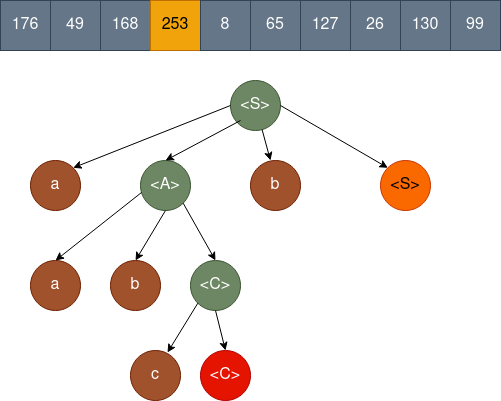
\includegraphics[scale=0.6]{parsing_tree_04.png}
	\caption{Genotype-phenotype mapping, step 4}
\end{figure}

Our current string is $a\:a\:b\:c\:{<}C{>}\:d\:{<}C{>}\:b\:{<}S{>}$, the index value is $i = 4$, and the codon value is $8$. The leftmost nonterminal symbol is ${<}C{>}$, which has $3$ productions defined. So we calculate $8\:\:MOD\:\:3\:=\:2$, and apply the production at index $2$, which is ${<}C{>}\:::=\:a$.

\begin{figure}[H]
	\centering
	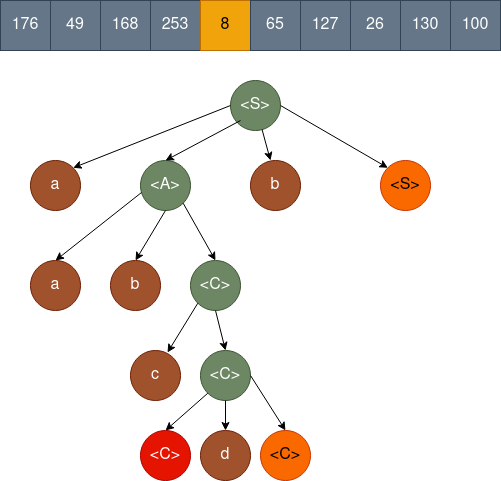
\includegraphics[scale=0.6]{parsing_tree_05.png}
	\caption{Genotype-phenotype mapping, step 5}
\end{figure}

Our current string is $a\:a\:b\:c\:a\:d\:{<}C{>}\:b\:{<}S{>}$, the index value is $i = 5$, and the codon value is $65$. The leftmost nonterminal symbol is ${<}C{>}$, which has $3$ productions defined. So we calculate $65\:\:MOD\:\:3\:=\:2$, and apply the production at index $2$, which is ${<}C{>}\:::=\:a$.

\begin{figure}[H]
	\centering
	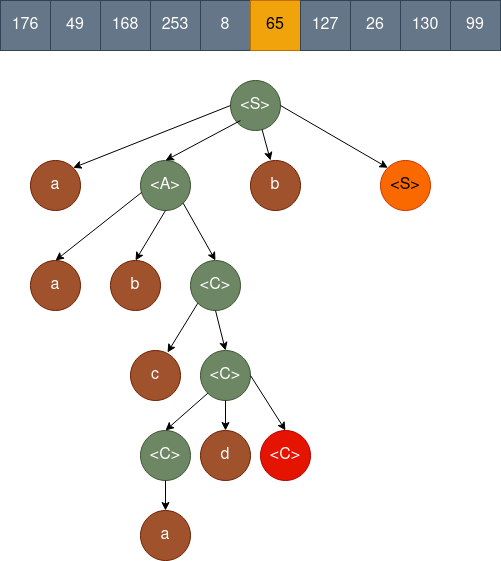
\includegraphics[scale=0.6]{parsing_tree_06.png}
	\caption{Genotype-phenotype mapping, step 6}
\end{figure}

Our current string is $a\:a\:b\:c\:a\:d\:a\:b\:{<}S{>}$, the index value is $i = 6$, and the codon value is $127$. The leftmost nonterminal symbol is ${<}S{>}$, which has $2$ productions defined. So we calculate $127\:\:MOD\:\:2\:=\:1$, and apply the production at index $1$, which is ${<}S{>}\:::=\:{<}C{>}\:d\:{<}A{>}$.

\begin{figure}[H]
	\centering
	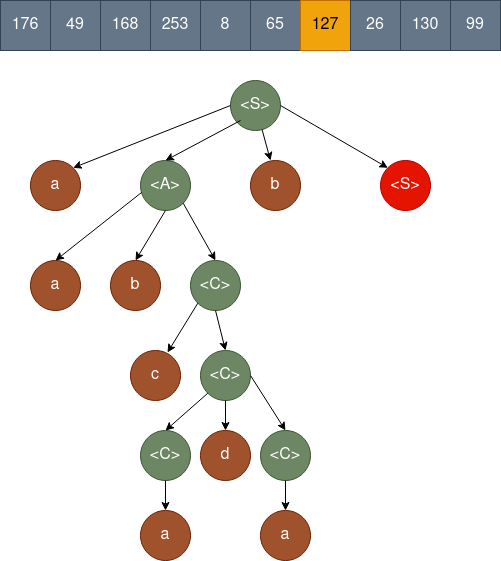
\includegraphics[scale=0.6]{parsing_tree_07.png}
	\caption{Genotype-phenotype mapping, step 7}
\end{figure}

Our current string is $a\:a\:b\:c\:a\:d\:a\:b\:{<}C{>}\:d\:{<}A{>}$, the index value is $i = 7$, and the codon value is $26$. The leftmost nonterminal symbol is ${<}C{>}$, which has $3$ productions defined. So we calculate $26\:\:MOD\:\:3\:=\:2$, and apply the production at index $2$, which is ${<}C{>}\:::=\:a$.

\begin{figure}[H]
	\centering
	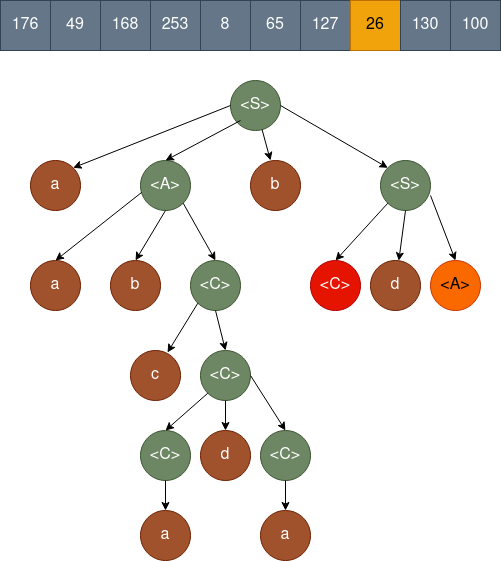
\includegraphics[scale=0.6]{parsing_tree_08.png}
	\caption{Genotype-phenotype mapping, step 8}
\end{figure}

Our current string is $a\:a\:b\:c\:a\:d\:a\:b\:a\:d\:{<}A{>}$, the index value is $i = 8$, and the codon value is $130$. The leftmost nonterminal symbol is ${<}A{>}$, which has $3$ productions defined. So we calculate $130\:\:MOD\:\:3\:=\:1$, and apply the production at index $1$, which is ${<}A{>}\:::=\:a\:b\:{<}C{>}$.

\begin{figure}[H]
	\centering
	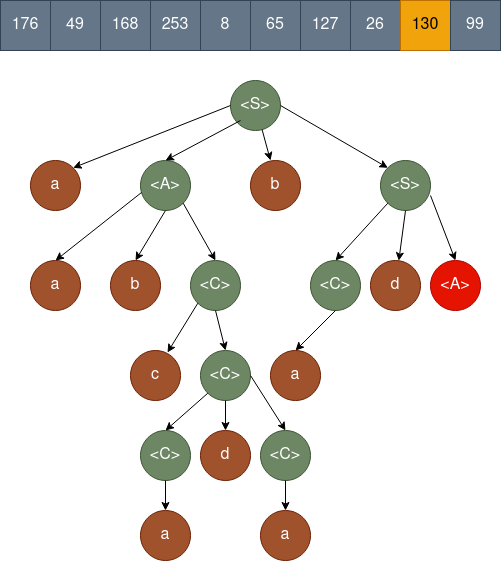
\includegraphics[scale=0.6]{parsing_tree_09.png}
	\caption{Genotype-phenotype mapping, step 9}
\end{figure}

Our current string is $a\:a\:b\:c\:a\:d\:a\:b\:a\:d\:a\:b\:{<}C{>}$, the index value is $i = 9$, and the codon value is $100$. The leftmost nonterminal symbol is ${<}C{>}$, which has $3$ productions defined. So we calculate $100\:\:MOD\:\:3\:=\:1$, and apply the production at index $1$, which is ${<}C{>}\:::=\:c\:{<}C{>}$.

\begin{figure}[H]
	\centering
	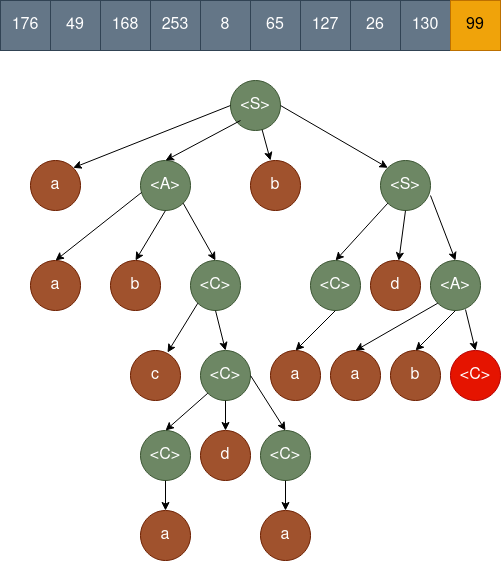
\includegraphics[scale=0.6]{parsing_tree_10.png}
	\caption{Genotype-phenotype mapping, step 10}
\end{figure}

Our current string is $a\:a\:b\:c\:a\:d\:a\:b\:a\:d\:a\:b\:c\:{<}C{>}$, the index value is $i = 10$. Since our codon array has only 10 elements, index $i = 10$ is out of bounds, but the mapping process is incomplete, so we apply the wrapping operator and set $i = 0$. The codon value is $176$. The leftmost nonterminal symbol is ${<}C{>}$, which has $3$ productions defined. So we calculate $176\:\:MOD\:\:3\:=\:2$, and apply the production at index $2$, which is ${<}C{>}\:::=\:a$.

\begin{figure}[H]
	\centering
	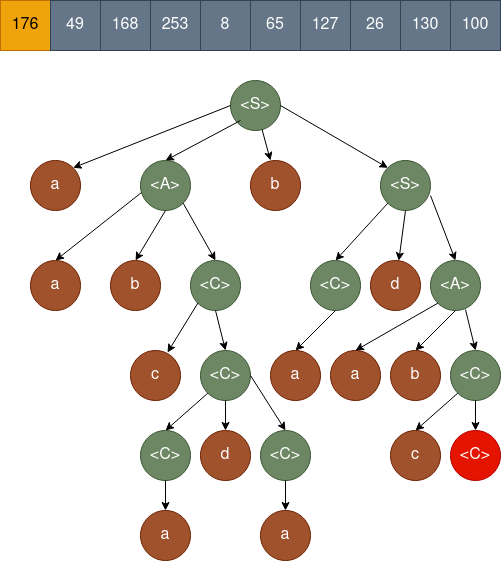
\includegraphics[scale=0.6]{parsing_tree_11.png}
	\caption{Genotype-phenotype mapping, step 11}
\end{figure}

Our current string is $a\:a\:b\:c\:a\:d\:a\:b\:a\:d\:a\:b\:c\:a$. Since there are no more nonterminal symbols in this string, the mapping process is finished, and this string is the final result of the mapping.

\begin{figure}[H]
	\centering
	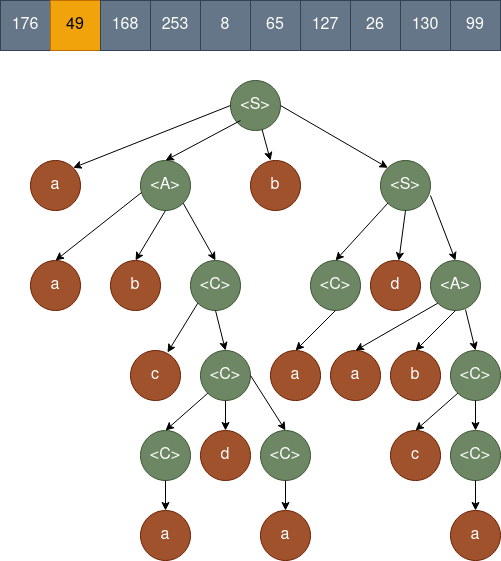
\includegraphics[scale=0.6]{parsing_tree_12.png}
	\caption{Genotype-phenotype mapping, step 12}
\end{figure}

\chapter{Evolving cache replacement policies}

\section{Cache replacement policies}
Paging is a memory management scheme that breaks up physical memory into fixed-size blocks called frames, and breaks up logical memory into same size blocks called pages \citep{silberschatz2018operatingsystem}. Physical memory refers to the real memory the operating system works with, and the logical memory refers to the memory space of each program being executed on the machine. Before a process is executed, it's pages are loaded into some frames.

Since the sum of logical spaces of all the programs being executed can exceed the physical space, sometimes a page must be kicked out of a frame, in order to make room for another page. This process is called swapping. The central question here is: which page should be kicked out? There are several strategies for this problem, and they are called cache replacement policies.

The FIFO (First In, First Out) strategy organizes the cache as a standard queue. The pages are kicked out in the order in which they were added.

The LRU (Least Recently Used) strategy kicks out the page which wasn't used for the longest time in the past. This strategy relies on the locality of reference, which means that if a page was recently accessed, it is likely that it will be accessed again in the near future.

The LFU (Least Frequently Used) strategy kicks out the page which was accessed the least number of times in some period of time.

The CLOCK strategy, also called the second chance strategy, traverses the frames in a round robin way. Each frame has a flag which can either have the value zero or one. When a page needs to be kicked out, the algorithm starts iterating over the frames, going to the first one once it reaches the end. If the current frame has the value of it's flag equal to zero, it's page is kicked out and the search is finished. If, on the other hand, it's flag is equal to one, the flag is set to zero, and the algorithm continues to the next frame, hence the 'second chance' name.

The general cache replacement policy looks as follows:

\begin{algorithm}[]
\caption{Cache replacement policy}
\begin{algorithmic}[1]
\State $\text{for each } \textit{page} \text{ in the requests array do}$
\State $\indent \text{if } \textit{page} \text{ in cache} $
\State $\indent \indent \text{do nothing;} $
\State $\indent \text{else if exists an empty } \textit{frame} $
\State $\indent \indent \text{put } \textit{page} \text{ in } \textit{frame;} $
\State $\indent \text{else} $
\State $\indent \indent \text{decide upon a } \textit{frame;}$
\State $\indent \indent \text{remove } \textit{current page} 
\text{ from } \textit{frame;}$
\State $\indent \indent \text{put } \textit{page} \text{ in } \textit{frame;} $
\State $\indent \text{end if}$
\State $\text{end while}$
\end{algorithmic}
\end{algorithm}

Lines 2 and 3 correspond to the situation where the currently required page is already in the cache. In that case, no action is needed.

Lines 4 and 5 correspond to the situation where the requested page isn't in the cache, but there exists an empty frame. In that case, we put the requested page in that empty frame.

Finally, lines 7, 8 and 9 correspond to the situation where teh requested page isn't in the cache, and all the frames already have some other page in them. In that case, first we must decide from which frame we will remove a page (line 7). Finally, we swap the old page from that frame with the requested page (lines 8 and 9).

An important note here is that all the cache replacement policies vary only in the line 7, that being the decision which frame will host the requested page. All other parts of the algorithm are equal in all strategies. 

When evolving cache replacement policies, we only change the line 7. Since the topic of this thesis is evolving these policies using grammatical evolution, the first step in this process is defining a grammar. This is a crucial step and the next subchapter will describe the constructed grammar in detail.

\section{Grammar for evolving cache replacement policies}
\subsection{Introduction to the grammar design}
Before listing and describing all the productions of our grammar, we will go through some of the nonterminal symbols, the building blocks of our strategies. It is also important to note that the implementation of this software system was written in the C++ language, so the grammar was written in a way that satisfies the C++ language rules. The architecure of the built software system is described in detail in the Appendix A.

\subsection{Nonterminal symbols}
The start symbol is ${<}block{>}$ and it corresponds to zero or more simpler statements, which are encapsulated in the ${<}statement{>}$ symbol. Each statement corresponds to a programming construct like a loop or a simple one line statement.

During the process of writing and fine-tuning the grammar, one of the problems was the possibility of loops occuring inside loops. This would drastically slow down the process of choosing a frame, which is a decision that should be made relatively quickly. To solve this problem, we will introduce the ${<}block\_no\_loop{>}$ and ${<}statement\_no\_loop{>}$ symbols. These symbols are semantically equivalent to ${<}block{>}$ and ${<}statement{>}$, except they won't be able to contains loops, and by introducing these symbols we will ensure that loops can't be nested.

Symbols ${<}expression{>}$ and ${<}term{>}$ will be used to generate simple expressions. The ${<}modifiable{>}$ symbol	 will agregate all terms which can go on the left and the right side of the equality operator '=', while the ${<}non\_modifiable{>}$ symbol will aggregate all terms which can go only on the right side of the equality operator.

Symbols ${<}bool{>}$ and ${<}number{>}$ will be used to generate constants.

\subsection{Information stored by each strategy}
Each strategy will keep track of some information about frames and pages, and this information will be available when choosing a frame in which the requested page will be stored. Each strategy will have four of these information arrays. The generated cache replacement policies will not manipulate these arrays directly, instead, each array will have some functions which are used to access it. In this sense, the function used to access the information arrays can be considered features ouf our learning problem.

The first array is called $last\_accessed$ and it keeps track of when each frame was last accessed. We will also introduce functions $last\_accessed\_min$ and $last\_accessed\_max$ which will return the index of the frame which was accessed least recently and most recently, respectively.

The second array is called $page\_access\_count$ and it keeps track of how many times each page was requested. We will introduce functions $page\_access\_count\_min$ and $page\_access\_count\_max$ which will return the index of the frame which holds the page that was accessed the least number of times and the most number of times, respectively.

The third array is called $added\_to\_cache$ and it keeps track of when each page was added to cache. We will introduce functions $added\_to\_cache\_min$ and $added\_to\_cache\_max$ which will return the index of the frame which holds the page that was added to cache least recently and most recently, respectively.

Finally, the fourth array is called $accessed$. The first function that manages this array is called $get\_accessed$. It takes one argument, the frame index, and returns the information stored about this frame. The second function is calles $set\_accessed$. It takes two arguments, the first being the index of the frame, and the second being some value, and it stores that value at the index of the frame in the accessed array. Each time a frame is accessed, its value is set to one. This array was introduced to make the implementation of the CLOCK strategy possible, as will be explained in subchapter 3.3. The unique feature of this array is that the generated strategies can change its contents, unlike the other arrays which are only changed automatically and the generated stragies can only read their contents.

Each strategy will also be given some arrays and variables which aren't updated automatically, instead, the strategy can use them to store whatever information it chooses. 

Each strategy will have two of these arrays, and they are accessed using the 'read' and 'write' functions. The read function takes two arguments, the first being the index of the array, and the second being the index (the frame number) in that array, and this function reads the value in that array at that index and returns it. The write function takes three arguments, the first being the index of the array, the second being the index (the frame number) in that array, and the third being the value that is being written at that index in that array.

Next to these two arrays, each strategy will also have three free variables which can they can change however they please, and these variables are called 'num1', 'num2' and 'num3'.

\subsection{Symbols ${<}block{>}$, ${<}block\_no\_loop{>}$}
The productions for the symbol ${<}block{>}$ look as follows:

\noindent
$ {<}block{>}\:::=\:{<}statement{>}\:{<}block{>}$\\
$ \indent\indent |\:""$

The first production allows recursive chaining of statements. The second production allows breaking the chaining, and without it, we would be stuck generating infinite statements one after another.

Similarly, productions for the ${<}block\_no\_loop{>}$ symbol are:

\noindent
$ {<}block\_no\_loop{>}\:::=\:{<}statement\_no\_loop{>}\:{<}block\_no\_loop{>}$\\
$ \indent\indent |\:""$

\subsection{Symbols ${<}statement{>}, {<}statement\_no\_loop{>}$}
Productions for the ${<}statement{>}$ symbol are:

\noindent
$ {<}statement{>}\:::=\:\text{if}\:\text{(}\:{<}expression{>}\:\text{)}\:\text{\{}\:{<}block{>}\:\text{\}}\:\text{else}\:\text{\{}\:{<}block{>}\:\text{\}} $\\
$ \indent\indent |\:\text{if}\:\text{(}\:{<}expression{>}\:\text{)}\:\text{\{}\:{<}block{>}\:\text{\}}$\\
$ \indent\indent |\:\text{iterations = 0;}\:\text{while}\:\text{(}\:{<}expression{>}\:\text{\&\& iterations < frame\_count}\:\text{)}\:\text{\{}\:\\{<}block\_no\_loop{>}\:\text{iterations++;}\:\text{\}} $\\
$ \indent\indent |\:{<}modifiable{>}\:\text{=}\:{<}term{>}\:\text{;} $\\
$ \indent\indent |\:\text{write}\:\text{(}\:{<}info\_field\_index{>}\:\text{,}\:{<}term{>}\:\text{,}\:\:{<}term{>}\:\text{)}\:\text{;} $\\
$ \indent\indent |\:\text{set\_accessed}\:\text{(}\:{<}term{>}\text{,}{<}term{>}\:\text{)}$

The first production generates simple if-else branches, while the second production generates if branches without the else part. The third production generates loops. Loops are written as while loops, which initialize the counter variable iterations to zero, and then the loop is executed while some expression is evaluated as true and the iteration count is smaller than the number of frames in the cache. After each iteration, the iterations variable is increased by one. The fourth production generates instructions with the equality operator. Finally, the fifth production generates calls of the 'write' function. This function is explained in the subchapter 3.2.3.

Similarly, productions for the ${<}statement\_no\_loop{>}$ symbol are:

\noindent
$ {<}statement\_no\_loop{>}\:::=\:\text{if}\:\text{(}\:{<}expression{>}\:\text{)}\:\text{\{}\:{<}block{>}\:\text{\}}\:\text{else}\:\text{\{}\:{<}block{>}\:\text{\}} $\\
$ \indent\indent |\:\text{if}\:\text{(}\:{<}expression{>}\:\text{)}\:\text{\{}\:{<}block{>}\:\text{\}}$\\
$ \indent\indent |\:{<}modifiable{>}\:\text{=}\:{<}term{>}\:\text{;} $\\
$ \indent\indent |\:\text{write}\:\text{(}\:{<}info\_field\_index{>}\:\text{,}\:{<}term{>}\:\text{,}\:\:{<}term{>}\:\text{)}\:\text{;} $\\
$ \indent\indent |\:\text{set\_accessed}\:\text{(}\:{<}term{>}\text{,}{<}term{>}\:\text{)}$

\subsection{Symbol ${<}expression{>}$}
Productions for the ${<}expression{>}$ symbol are:

\noindent
$ {<}expression{>}\:::=\:{<}term{>} $\\
$ \indent\indent |\:{<}term{>}\:\text{==}\:{<}term{>} $\\
$ \indent\indent |\:{<}term{>}\:\text{!=}\:{<}term{>} $\\
$ \indent\indent |\:{<}term{>}\:\text{>}\:{<}term{>} $\\
$ \indent\indent |\:{<}term{>}\:\text{>=}\:{<}term{>} $\\
$ \indent\indent |\:{<}term{>}\:\text{<}\:{<}term{>} $\\
$ \indent\indent |\:{<}term{>}\:\text{<=}\:{<}term{>} $\\
$ \indent\indent |\:{<}term{>}\:\text{+}\:{<}term{>} $\\
$ \indent\indent |\:{<}term{>}\:\text{-}\:{<}term{>} $\\
$ \indent\indent |\:{<}term{>}\:\text{*}\:{<}term{>} $\\
$ \indent\indent |\:\text{division}\:\text{(}\:{<}term{>}\:\text{,}\:\:{<}term{>}\:\text{)} $\\
$ \indent\indent |\:\text{remainder}\:\text{(}\:{<}term{>}\:\text{,}\:\:{<}term{>}\:\text{)} $

All of these productions generate simple arithmetic expressions. The division and remainder operators are written as functions, rather than just operators, because we will encapsulate these operations into functions that safely handle division by zero.

\subsection{Symbol ${<}term{>}$}
Productions for the ${<}term{>}$ symbol are:

\noindent
$ {<}term{>}\:::=\:{<}modifiable{>} $\\
$ \indent\indent |\:{<}non\_modifiable{>} $\\
$ \indent\indent |\:{<}expression{>} $

The ${<}term{>}$ symbol occurs inside expressions and it generates modifiable variables (which can be on the left and the right side of the equality operator), non-modifiable variables (which can only be on the right side of the equality operator), constants and nested expressions.

\subsection{Symbol ${<}modifiable{>}$}
Productions for the ${<}modifiable{>}$ symbol are:

\noindent
$ {<}modifiable{>}\:::=\:\text{frame} $\\
$ \indent\indent |\:\text{num1} $\\
$ \indent\indent |\:\text{num2} $\\
$ \indent\indent |\:\text{num3} $

We have already established that our strategies will only evolve the line 7 in the Algorithm 2, that being the decision in which frame should we put the page that isn't currently in the cache if all the frames are taken. For the sake of convenience, we will model this with functions that initialize the frame variable to zero and return that frame variable. The frame variable corresponds to the index of the chosen frame. We will want our strategies to modify this variable from its initial value of zero, and that's why this variable will be modifiable. The 'num1', 'num2' and 'num3' variables are the free variables of the each strategy, and they are explained in the subchapter 3.2.3.

\subsection{Symbol ${<}non\_modifiable{>}$}
Productions for the ${<}non\_modifiable{>}$ symbol are:

\noindent
$ {<}non\_modifiable{>}\:::=\:\text{time} $\\
$ \indent\indent |\:\text{cache\_size} $\\
$ \indent\indent |\:\text{page\_request} $\\
$ \indent\indent |\:\text{find\_min}\:\text{(}\:{<}info\_field\_index{>}\:\text{)} $\\
$ \indent\indent |\:\text{find\_max}\:\text{(}\:{<}info\_field\_index{>}\:\text{)} $\\
$ \indent\indent |\:\text{read}\:\text{(}\:{<}info\_field\_index{>}\:\text{,}\:{<}term{>}\:\text{)} $\\
$ \indent\indent |\:\text{page\_access\_count\_min}\:\text{(}\:\text{)}$\\
$ \indent\indent |\:\text{page\_access\_count\_max}\:\text{(}\:\text{)}$\\
$ \indent\indent |\:\text{last\_accessed\_min}\:\text{(}\:\text{)}$\\
$ \indent\indent |\:\text{last\_accessed\_max}\:\text{(}\:\text{)}$\\
$ \indent\indent |\:\text{added\_to\_cache\_min}\:\text{(}\:\text{)}$\\
$ \indent\indent |\:\text{added\_to\_cache\_max}\:\text{(}\:\text{)}$\\
$ \indent\indent |\:\text{get\_accessed}\:\text{(}\:{<}term{>}\:\text{)}$\\
$ \indent\indent |\:{<}number{>} $\\
$ \indent\indent |\:{<}bool{>} $

The variable time refers to the index of the current request, and it gets increased by one for each new request. The variable cache\_size refers to the number of frames in the cache, and the page\_request variable refers to the page index of the page that is currently being requested. Function find\_min takes one input argument, which is the index of strategy's arrays (and it can be one or two since each strategy has two info arrays), and it returns the index at which this array has the minimal vaue. The function find\_max works in a similar way, except it returns the index at which the array has the maximal value. The rest of the productions are explained in the subchapters 3.2.2. and 3.2.3.

\subsection{Symbol ${<}bool{>}$}
Productions for the ${<}bool{>}$ symbol are:

\noindent
$ {<}bool{>}\:::=\:\text{true} $\\
$ \indent\indent |\:\text{false} $

This symbol generates elementary Boolean logic constants, true and false.

\subsection{Symbol ${<}info\_field\_index{>}$}
Productions for the ${<}info\_field\_index{>}$ symbol are:

\noindent
$ {<}info\_field\_index{>}\:::=\:\text{1} $\\
$ \indent\indent |\:\text{2} $

As it was already explained, each strategy has two info arrays in which they can store arbitrary information about each frame. Addressing these info arrays is done using this symbol.

\subsection{Symbols ${<}number{>}$, ${<}first\_digit{>}$, ${<}tail\_digits{>}$, ${<}digit{>}$}
Finally, the symbols for generating integer constants are ${<}number{>}$, ${<}first\_digit{>}$, ${<}tail\_digits{>}$ and ${<}digit{>}$. Productions for generating numbers are recursive, and they can't start with the digit zero (unless the number is zero), since we want these numbers to be written in the decimal base, and if a number starts with 0 in the C++ language, it is interpreted as an octal number. Productions for these symbols are:

\noindent
$ {<}number{>}\:::=\:{<}first\_digit{>}\:{<}tail\_digits{>}\:|\:\text{0} $\\
$ {<}first\_digit{>}\:::=\:\text{1}\:|\:\text{2}\:|\:\text{3}\:|\:\text{4}\:|\:\text{5}\:|\:\text{6}\:|\:\text{7}\:|\:\text{8}\:|\:\text{9} $\\
$ {<}tail\_digits{>}\:::=\:{<}digit{>}\:{<}tail\_digits{>}\:|\:"" $\\
$ {<}digit{>}\:::=\:\text{0}\:|\:\text{1}\:|\:\text{2}\:|\:\text{3}\:|\:\text{4}\:|\:\text{5}\:|\:\text{6}\:|\:\text{7}\:|\:\text{8}\:|\:\text{9} $

\input{Classic_Strategies_As_Grammar}

\chapter{Experimental results}

\chapter{Conclusion}

The goal of this thesis was to explore grammatical evolution as a grammar-based approach to genetic programming, study the problem of managing cache in modern computer systems, implement a software system capable of evolving valid computer programs in an arbitrary language which solve an arbitrary problem, use the built software system to generate and evolve cache replacement policies using real objective train data, test the generated strategies using real objective test data, and compare the generated strategies against the classic heuristic approaches to solving the cache management problem on different cache sizes.

Grammatical evolution has proven able to generate cache replacement policies which can match classic heuristic approaches for solving this problem. For future work, it would be interesting to see how different derivatives and improved versions of this algorithm would compare against the simple version of the algorithm used in this thesis.

\bibliography{literatura}
\bibliographystyle{fer}


\appendix
\chapter{Software architecture}

For the purposes of writing this thesis, an implementation of the grammatical evolution algorithm was developed using the object-oriented paradigm in the C++ language. This system can be used to generate and evolve programs in any arbitrary language, used to solve any arbitrary problem.

The classes written for this generic part of the implementation are:

\begin{list}{$\bullet$}{}  	
	\item \textbf{GrammaticalEvolution} - the top class in the hierarchy, used to encapsulate the process of mapping a unit's genotype onto its phenotype
	\item \textbf{Grammar} - the class used for reading and parsing the .bnf files, and also storing information about a grammar and its productions 
	\item \textbf{Crossover} - an implementation of the crossover operator
	\item \textbf{Mutation} - an implementation of the mutation operator
	\item \textbf{Unit} - the class used for storing information about a unit
	\item \textbf{Node} - the process of the genotype-phenotype mapping is implemented using linked lists, and this class encapsulates nodes in this list
	\item \textbf{Symbol} - a class used in the genotype-phenotype mapping, stores information about the contents of each node in the linked list
	\item \textbf{GrammarParsingState} - the process of reading and parsing the .bnf file is implemented as a final automata, and this enumeration stores all the states of that automata
	\item \textbf{SymbolType} - an enumeration which stores all types which and instance of the class Symbol can have, and the types are terminal and non-terminal
	\item \textbf{DecodeException} - a class used for handling all potential problems during the process of parsing a .bnf file
\end{list}

The other part of the implementation is the classes used for the purpose of evolving cache replacement policies. These classes are:

\begin{list}{$\bullet$}{}  	
	\item \textbf{Strategy} - the base class for a cache replacement strategy
	\item \textbf{GEStrategy} - the class used for the strategies generated by the GrammaticalEvolution
	\item \textbf{GeneratedStrategies} - the class which stores all generated strategies in one place; this class has to be recompiled during each iteration of the genetic algorithm
	\item \textbf{FIFO} - an implementation of the FIFO strategy
	\item \textbf{LRU} - an implementation of the LRU strategy
	\item \textbf{LFU} - an implementation of the LFU strategy
	\item \textbf{CLOCK} - an implementation of the CLOCK strategy
	\item \textbf{OPT} - an implementation of the OPT strategy
\end{list}

For the sake of simplicity and the adherence to the 'separation of concerns' principle, the main function was split into six files, each with its own main function. These files are:

\begin{list}{$\bullet$}{}  	
	\item \textbf{init} - initializes a random population and stores each unit's genotype in a separate file inside the /solutions directory
	\item \textbf{decode} - reads the genotypes of every unit inside the current population and decodes their genotypes to their phenotypes, which are then stored inside the GeneratedStrategies
	\item \textbf{run} - tests all strategies from the GeneratedStrategies using the train data, and stores their scores inside the /results directory
	\item \textbf{evolution} - reads each strategy's score and performs the evolutionary process of creating a new generation, which is then stored inside the /solutions directory
	\item \textbf{test\_generated} - simulates a generated strategy using the test data and outputs its hit count
	\item \textbf{test\_heuristic\_strategies} - simulates the heuristic stragies using the test data and outputs their hit counts
\end{list}

During each iteration of the evolutionary process, new strategies are generated and stored as C++ files, which need to be compiled before they can be run. The class responsible for decoding the genotype of each unit, which is an array of 8-bit numbers, to its corresponding phenotype, which is a computer program, is the GrammaticalEvolution class. This class has a decode method which takes as input some Unit and returns its phenotype representation as a string. This string needs to be carefully placed into a specific file, so that it can be correctly compiled and run. This is the responsibility of the main loop of the program. This main loop isn't written as a C++ file, instead it is a bash script. This bash script manages and calls the six files which do a specific part of the evolutionary process, recompiles the parts of the code that change during each iteration, and assures the persistency of the generated strategies between each run. Each strategy has a genotype, phenotype and score, and each of these is stored inside a different textual file.

Figure A.1 shows a class diagram of the complete project. The classes which belong to the core part of the project and which can be applied to any problem are colored in blue. The classes which are specificly built for the problem of evolving cache replacement strategies are colored in green. These classes are shown without their member variables and functions since these are unimportant in viewing the whole project and the connections between its parts. Finally, the six C++ files which are being compiled to executable programs and subsequently run by the main bash script are colored in yellow. These aren't classes so they technically don't belong in a class diagram, but they were included for the sake of showing all the built components and their connections. The diagram was built using the tool \citep{diagrams}.

\begin{figure}[H]
	\centering
	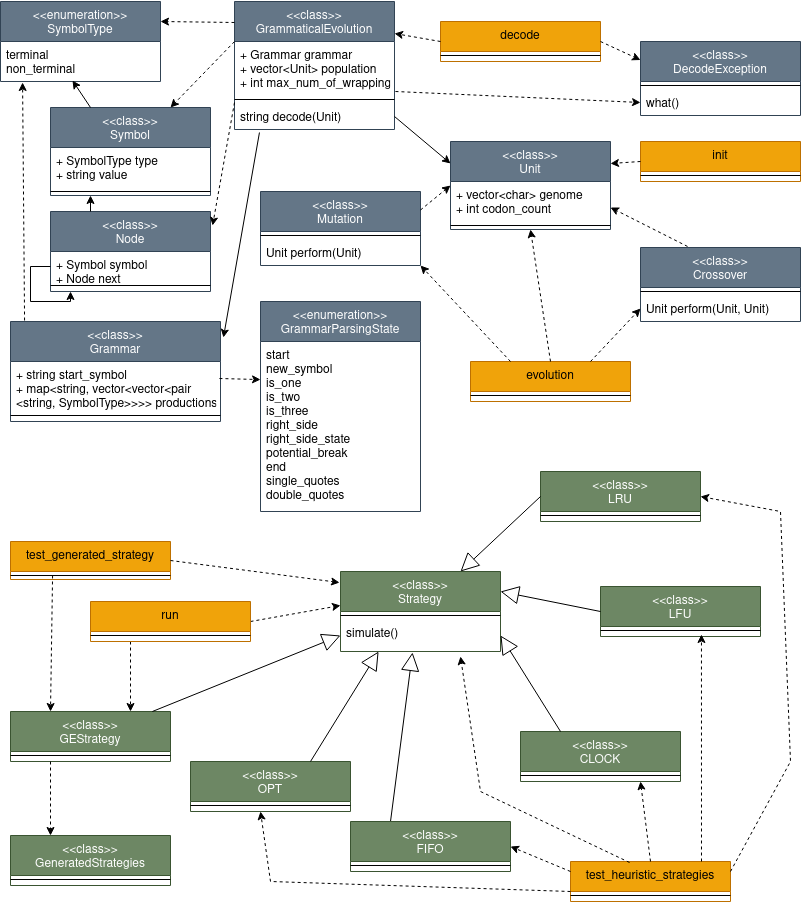
\includegraphics[scale=0.55]{class_diagram.png}
	\caption{Class diagram}
\end{figure}


\begin{sazetak}
Sažetak na hrvatskom jeziku.

\kljucnerijeci{Ključne riječi, odvojene zarezima.}
\end{sazetak}

% TODO: Navedite naslov na engleskom jeziku.
\engtitle{Title}
\begin{abstract}
Abstract.

\keywords{Keywords.}
\end{abstract}

\end{document}